\documentclass[fleqn,12pt]{article}
\usepackage{mycommands,amssymb,amsmath,amsthm,color,pagesize,outlines,cite,caption}
\usepackage[pdftex]{graphicx}
\usepackage[round]{natbib}
\addtolength{\evensidemargin}{-.5in}
\addtolength{\oddsidemargin}{-.5in}
\addtolength{\textwidth}{0.9in}
\addtolength{\textheight}{0.9in}
\addtolength{\topmargin}{-.4in}

\usepackage{hyperref} % for linking references 
\usepackage{setspace}
\doublespacing

%\DeclareMathOperator*{\vec}{vec}

\begin{document}

\newtheorem{Theorem}{Theorem}[section]
\newtheorem{Lemma}[Theorem]{Lemma}
\newtheorem{Corollary}[Theorem]{Corollary}

\title{Robust estimation of principal components from depth-based multivariate rank covariance matrix}
\date{}
\author{Subho Majumdar}
\maketitle

Abstract:
Analyzing principal components for multivariate data from its spatial sign covariance matrix (SCM) has been proposed as a computationally simple and robust alternative to normal PCA, but it suffers from poor efficiency properties and is actually inadmissible with respect to the maximum likelihood estimator. Here we use data depth-based spatial ranks in place of spatial signs to obtain the orthogonally equivariant Depth Covariance Matrix (DCM) and use its eigenvector estimates for PCA. We derive asymptotic properties of the sample DCM and influence functions of its eigenvectors. The shape of these influence functions indicate good efficiency properties compared to the SCM. Finite sample simulation studies show that principal components of the sample DCM are robust with respect to deviations from normality and infinitesimal contamination, as well as are more efficient than the SCM.

Keywords:
Data depth; Principal components analysis; Robustness; Sign covariance matrix; Multivariate ranking

\section{Introduction}

\section{Preliminaries}

\section{Depth-based rank covariance matrix}

Consider a vector-valued random variable $\bfX \in \mathbb{R}^p$ that follows an elliptic distribution $|\Sigma|^{-1/2} f((\bfx - \bfmu)^T \Sigma^{-1} (\bfx - \bfmu))$, with a mean vector $\bfmu$ and covariance matrix $\Sigma$. Now, given a depth function $D_{\bfX}(\bfx)$ (equivalently, an htped function $\tilde D_\bfX(\bfx)$), transform the original random variable as: $\tilde \bfx = \tilde D_\bfX(\bfx) \bfS(\bfx - \bfmu)$, $\bfS(.)$ being the spatial sign functional:

$$ \bfS(\bfx) = \begin{cases} \bfx\| \bfx \|^{-1} \quad \mbox{if }\bfx \neq \bf0\\
\bf0 \quad \mbox{if }\bfx = \bf0 \end{cases} $$

The sign transformation is rotation equivariant, in the sense that $ \bfS(P \bfx) = P\bfx/\| P \bfx \| = P\bfx/\| \bfx \| = P \bfS(\bfx)$ for any orthogonal matrix $P$. The transformed random variable $\tilde \bfX$ can be seen as the multivariate rank corresponding to $\bfX$ (e.g. \cite{serfling2006}).

\begin{figure}[t]
	\captionsetup{singlelinecheck=off}
	\centering
		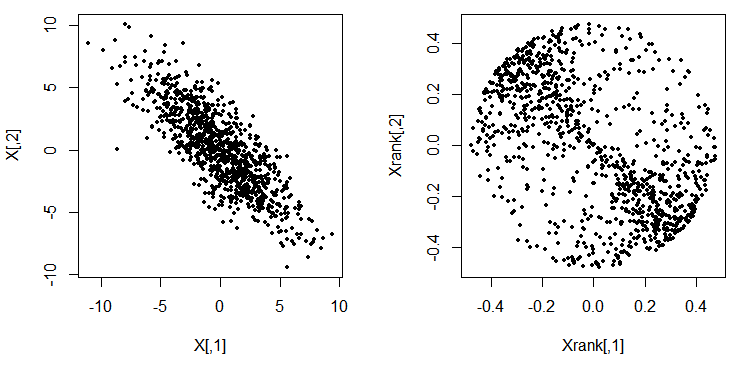
\includegraphics[height=5cm]{../Codes/rankplot.png}
	\caption{(Left) 1000 points randomly drawn from $\mathcal N_2\left((0,0)^T, \left(\protect\begin{smallmatrix} 5 & -4 \\ -4 & 5 \protect\end{smallmatrix}\right)\right) $ and (Right) their multivariate ranks based on halfspace depth}
	\label{fig:rankplot}
\end{figure}

Now, consider the spectral decomposition of the covariance matrix: $\Sigma = \Gamma\Lambda\Gamma^T$, $\Gamma$ being orthogonal and $\Lambda$ diagonal with positive diagonal elements. Also normalize the original random variable as $\bfz = \Gamma^T\Lambda^{-1/2} (\bfx - \bfmu)$. In this setup, we can represent the transformed random variable as
\begin{eqnarray*}
\tilde \bfx &=& \tilde D_{\bfX} (\bfx) \bfS(\bfX - \bfmu)\\
&=& \tilde D_{\Gamma\Lambda^{1/2}\bfZ + \bfmu} (\Gamma\Lambda^{1/2} \bfz + \bfmu). \bfS(\Gamma\Lambda^{1/2} \bfz)\\
&=& \Gamma \tilde D_{\bfZ}(\bfz) \bfS(\Lambda^{1/2}\bfz)\\
&=& \Gamma \Lambda^{1/2} \tilde D_{\bfZ}(\bfz) \bfS(\bfz) \frac{\| \bfz \|}{\|\Lambda^{1/2} \bfz\|}
\end{eqnarray*}

%Because of affine (thus rotational) invariance of a depth function, the depth (htped) value at $\bfz$ does not depend on the direction of $\bfz$, i.e. $\tilde D_{\bfZ}(\bfz)$ and $\bfS(\bfz)$ are independent. Furthermore,
%$$ Cov \left(\bfS (\bfz), \frac{\| \bfz \|}{\|\Lambda^{1/2} \bfz\|} \right) = E \left(\bfS (\bfz). \frac{\| \bfz \|}{\|\Lambda^{1/2} \bfz\|} \right) - E \bfS (\bfz) E \left(\frac{\| \bfz \|}{\|\Lambda^{1/2} \bfz\|} \right) = E \left( \frac{\bfz}{\|\Lambda^{1/2} \bfz\|} \right) = \bf0$$
%both $\bfS (\bfz)$ and $\bfz / \| \Lambda^{1/2}\bfz \|$ are odd functions of $\bfz$, which has a circularly symmetric distribution, hence each of them has expectation $\bf0$. Consequently, we obtain an expression for the covariance matrix of $\tilde \bfX$:

$\tilde D_\bfZ(\bfz)$ is an odd function in $\bfz$ because of affine invariance, as is $\| \bfz \| / \|\Lambda^{1/2} \bfz \|$. Since $\bfS(\bfz)$ is odd in $\bfz$ for circularly symmetric $\bfz$, it follows that $E(\tilde \bfX) = \bf0$, and consequently we obtain an expression for the covariance matrix of $\tilde \bfX$:

\begin{Theorem} \label{Theorem:covform}
Let the random variable $\bfX \in \mathbb{R}^p$ follow an elliptical distribution with center $\bfmu$ and covariance matrix $\Sigma = \Gamma\Lambda\Gamma^T$, its spectral decomposition. Then, given a depth function $D_\bfX(.)$ the covariance matrix of the transformed random variable $\tilde\bfX$ is
\begin{equation} \label{equation:covformEq1}
Cov(\tilde \bfX) = \Gamma \Lambda_{D,S} \Gamma^T,\quad\mbox{with}\quad \Lambda_{D,S} = E \left[ (\tilde D_\bfZ(\bfz))^2 \frac{\Lambda^{1/2} \bfz \bfz^T \Lambda^{1/2}}{\bfz^T \Lambda \bfz} \right]
\end{equation}

where $\bfz = (z_1,...,z_p)^T \sim N({\bf 0}, I_p)$ and $\Lambda_{D,S}$ a diagonal matrix with diagonal entries

$$ \lambda_{D,S,i} = E_\bfZ \left[ \frac{(\tilde D_\bfZ(\bfz))^2 \lambda_i z_i^2}{\sum_{j=1}^p \lambda_j z_j^2} \right] $$
\end{Theorem}

The matrix of eigenvectors of the covariance matrix, $\Gamma$, remains unchanged in the transformation $\bfX \rightarrow \tilde \bfX$. As a result, the multivariate rank vectors can be used for robust principal component analysis, which will be outlined in the following sections. However, as one can see in the above expression, the diagonal entries of $\Lambda_{D,S}$ do not change if a scale change is done on all entries of $\Lambda$, meaning the $\Lambda_{D,S}$ matrices corresponding to $F$ and $cF$ for some $c \neq 0$ will be same. This is the reason for lack of affine equavariance of the DCM. Following the case of multivariate sign covariance matrices \citep{taskinen12} one can get back the shape components, i.e. original \textit{standardized} eigenvalues $\Lambda^*$ from $\Lambda_{D,S}$ by an iterative algorithm:

\begin{enumerate}
\item Set $k=0$, and start with an initial value $\Lambda^{*(0)}$.

\item Calculate the next iterate
$$ \Lambda^{*(k+1)} = \left[ E\left( \frac{(\tilde D_\bfZ(\bfz))^2 \bfz \bfz^T}{\bfz^T \Lambda^{*(k)} \bfz} \right) \right]^{-1} \Lambda_{D,S} $$

and standardize its eigenvalues:
$$ \Lambda^{*(k+1)} = \frac{\Lambda^{*(k+1)}}{det(\Lambda^{*(k+1)})^{1/p}} $$

\item Stop if convergence criterion is satisfied. Otherwise set $k \rightarrow k+1$ ad go to step 2.
\end{enumerate}

Unlike sign covariance matrices and symmetrized sign covariance matrices \citep{dumbgen98}, however, attempting to derive an affine equivariant counterpart (as opposed to only orthogonal equivariance) of the DCM through an iterative approach analogous to \cite{tyler87} will not result in anything new. This is because Tyler's scatter matrix $\Sigma_T$ is defined as the implicit solution to the following equation:
\begin{equation} \label{equation:tylerEq}
\Sigma_T = \frac{\bfx \bfx^T}{\bfx^T \Sigma_T^{-1} \bfx}
\end{equation}

and simply replacing $\bfx$ by its multivariate rank counterpart $\tilde\bfx$ will not change the estimate $\Sigma_T$ as $\bfx$ and $\tilde \bfx$ have the same directions. Instead we consider a depth-weighted version of Tyler's scatter matrix (i.e. weights $(\tilde D_\bfX(\bfx))^2$ in right side of (\ref{equation:tylerEq})) in the simulations in Section \ref{section:simSection}. The simulations show that it has slightly better finite-sample efficiency than $\Sigma_T$ but has same asymptotic performance. We conjecture that its concentration properties can be obtained by taking an approach similar to \cite{soloveychik14}.

\section{Asymptotic results}
\subsection{The sample DCM}
Let us now consider $n$ iid random draws from our elliptic distribution $F$, say $\bfX_1,...,\bfX_n$. For ease of notation, denote $SS(\bfx; \bfmu) = \bfS(\bfx - \bfmu) \bfS(\bfx - \bfmu)^T$. Then, given the depth function and known location center $\bfmu$, one can show that the sample DCM $\sum_{i=1}^n (\tilde D_\bfX(\bfx_i))^2SS(\bfx_i; \bfmu) /n$ is a $\sqrt n$-consistent estimator of $E[( (\tilde D_\bfX (\bfX))^2 SS(\bfx; \bfmu)]$ by a straightforward application of CLT. But in practice the population depth function $D_\bfX(\bfx) = D(\bfx, F)$ is estimated by the depth function based on the empirical distribution function, $F_n$. Denote this sample depth by $D^n_\bfX (\bfx) = D(\bfx, F_n)$. One also needs to replace the known location parameter $\bfmu$ by some estimator $\hat\bfmu_n$. Examples of robust estimators of location that are relevant here include the spatial median \citep{haldane48,brown83}, Oja median \citep{oja83}, projection median \citep{zuo03} etc. Now, given $D^n_\bfX(.)$ and $\hat \bfmu_n$, to plug them into the sample DCM and still go through with the consistency we need the following result:

\begin{Lemma} \label{Lemma:lemma1}
Consider a random variable $\bfX \in \mathbb{R}^p$ having a continuous and symmetric distribution with location center $\bfmu$ such that $E\|\bfx - \bfmu \|^{-3/2} < \infty$. Given $n$ random samples from this distribution, suppose $\hat\bfmu_n$ is an estimator of $\bfmu$ so that $\sqrt n (\hat\bfmu_n - \bfmu) = O_P(1) $. Then with the above notations, and given that $D^n_\bfX (\bfx) \stackrel{P}{\rightarrow} D_\bfX (\bfx)$,

$$ \sqrt n \left[
\frac{1}{n} \sum_{i=1}^n (\tilde D^n_\bfX (\bfx_i))^2 SS(\bfx_i; \hat\bfmu_n) -
\frac{1}{n} \sum_{i=1}^n (\tilde D_\bfX (\bfx_i))^2 SS(\bfx_i; \bfmu) \right]
\stackrel{P}{\rightarrow} 0 $$
\end{Lemma}

Given this lemma, we can now state the result for consistency of the sample DCM:

\begin{Theorem} \label{Theorem:rootn}
Consider $n$ iid samples from the distribution in Lemma \ref{Lemma:lemma1}. Then, given a depth function $D_\bfX(.)$ and an estimate of center $\hat\bfmu_n$ so that $\sqrt n(\hat \bfmu_n - \bfmu) = O_P(1)$,

$$ \sqrt n \left[ vec\left\{ \frac{1}{n} \sum_{i=1}^n (\tilde D^n_\bfX (\bfx_i))^2 SS(\bfx_i; \hat\bfmu_n) \right\} - E \left[ vec\left\{ (\tilde D_\bfX (\bfx))^2 SS(\bfx; \bfmu) \right\} \right] \right]
\stackrel{D}{\rightarrow}
N_{p^2} ({\bf 0}, V_{D,S}(F)) $$
$$ \text{with } V_{D,S}(F) = Var \left[vec \left\{ (\tilde D_\bfX (\bfx))^2 SS(\bfx; \bfmu) \right\} \right] $$
\end{Theorem}

In case $F$ is elliptical, an elaborate form of the covariance matrix $V_{D,S}(F)$ explicitly specifying each of its elements (more directly those of its $\Gamma^T$-rotated version) can be obtained, which is given in Appendix A. This form is useful when deriving limiting distributions of eigenvectors and eigenvalues of the sample DCM.

\subsection{Eigenvectors and eigenvalues} Since we are mainly interested in using the DCM for a robust version of principal components analysis, from now on we assume that the eigenvalues of $\Sigma$ are distinct: $\lambda_1 > \lambda_2 > ... > \lambda_p$ to obtain asymptotic distributions of principal components. In the case of eigenvalues with larger than 1 multiplicities, the limiting distributions of eigenprojection matrices can be obtained analogous to those of the sign covariance matrix \citep{magyar14}.

\paragraph{}We are going to derive the asymptotic joint distributions of eigenvectors and eigenvalues of the sample DCM. The following result allows us to get these, provided we know the limiting distribution of the sample DCM itself:

\begin{Theorem} \label{Theorem:decomp} \citep{taskinen12}
Let $F_\Lambda$ be an elliptical distribution with a diagonal covariance matrix $\Lambda$, and $\hat C$ be any positive definite symmetric $p \times p$ matrix such that at $F_\Lambda$ the limiting distribution of $\sqrt n vec(\hat C - \Lambda)$ is a $p^2$-variate (singular) normal distribution with mean zero. Write the spectral decomposition of $\hat C$ as $\hat C = \hat P \hat\Lambda \hat P^T$. Then the limiting distributions of $\sqrt n vec(\hat P - I_p)$ and $\sqrt n vec(\hat\Lambda - \Lambda)$ are multivariate (singular) normal and
\begin{equation} \label{equation:decompEq}
\sqrt n vec (\hat C - \Lambda)  = \left[ (\Lambda \otimes I_p) - (I_p \otimes \Lambda) \right] \sqrt n vec (\hat P - I_p) + \sqrt n vec (\hat\Lambda - \Lambda) + o_P(1)
\end{equation}
\end{Theorem}

The first matrix picks only off-diagonal elements of the LHS and the second one only diagonal elements. We shall now use this as well as the form of the asymptotic covariance matrix of the vec of sample DCM, i.e. $V_{D,S}(F)$ to obtain limiting variance and covariances of eigenvalues and eigenvectors.

\begin{Corollary} \label{Corollary:eigendist}
Consider the sample DCM $ \hat S^D(F) = \sum_{i=1}^n (\tilde D^n_\bfX (\bfx_i))^2 SS(\bfx_i; {\bf \hat\bfmu_n})/n $ and its spectral decomposition $\hat S^D(F) = \hat\Gamma_D \hat\Lambda_D \hat\Gamma_D^T $. Then the matrices $G = \sqrt n (\hat\Gamma_D - \Gamma) $ and $L = \sqrt n (\hat\Lambda_D - \Lambda_{D,S}) $ have independent distributions. $vec(G)$ asymptotically has a $p^2$-variate normal distribution with mean ${\bf 0}_{p^2}$, and the asymptotic variance and covariance of different columns of $G = (\bfg_1,...,\bfg_p)$ are as follows:
\begin{equation} \label{equation:DevEq}
AVar(\bfg_i) = \sum_{k=1; k \neq i}^p \frac{1}{(\lambda_{D,s,k} - \lambda_{D,S,i})^2} E \left[ \frac{(\tilde D_\bfZ (\bfz))^4 \lambda_i \lambda_k z_i^2 z_k^2}{(\bfz^T \Lambda \bfz)^2} \right] \bfgamma_k \bfgamma_k^T
\end{equation}
\begin{equation}
ACov(\bfg_i, \bfg_j) = - \frac{1}{(\lambda_{D,s,i} - \lambda_{D,S,j})^2} E \left[ \frac{(\tilde D_\bfZ (\bfz))^4 \lambda_i \lambda_j z_i^2 z_j^2}{(\bfz^T \Lambda \bfz)^2} \right] \bfgamma_j \bfgamma_i^T; \quad i \neq j
\end{equation}

where $\Gamma = (\bfgamma_1,...,\bfgamma_p)$. The vector consisting of diagonal elements of $L$, say $\bfl = (\l_1,...,\l_p)^T$ asymptotically has a $p$-variate normal distribution with mean ${\bf 0}_p$ and variance-covariance elements:
\begin{eqnarray}
AVar(l_i) &=& E \left[ \frac{(\tilde D_\bfZ (\bfz))^4 \lambda_i^2 z_i^4}{(\bfz^T \Lambda \bfz)^2} \right] - \lambda_{D,S,i}^2\\
ACov(l_i, l_j) &=& E \left[ \frac{(\tilde D_\bfZ (\bfz))^4 \lambda_i \lambda_j z_i^2 z_j^2}{(\bfz^T \Lambda \bfz)^2} \right] - \lambda_{D,S,i} \lambda_{D,S,j}; \quad i \neq j
\end{eqnarray}

\end{Corollary}

\section{Robustness and efficiency properties} \label{section:simSection}
In this section, we first obtain the influence functions of the DCM as well as its eigenvectors and eigenvalues, which are essential to understand how much influence a sample point, especially an infitesimal contamination, has on any functional on the distribution \citep{hampel}. We shall also derive the asymptotic efficiencies of individual principal components with respect to those of the original covariance matrix and sign covariance matrix. Unlike affine equivariant estimators of shape, the ARE of eigenvectors (with respect to any other affine equivariant estimator) can not be simplified as a ratio of two scalar quantities dependent on only the distribution of $\| \bfz \|$ (e.g. \cite{taskinen12,ollilia03}). Finite sample efficiency of the DCM estimates with respect to infitesimal contamination and heavy-tailed distributions shall also be demonstrated by a simulation study.

\subsection{Influence functions}
Given any probability distribution $F$, the influence function of any point $\bfx_0$ in the sample space $\mathcal{X}$ for some functional $T(F)$ on the distribution is defined as

$$ IF(\bfx_0; T,F) = \lim_{\epsilon \rightarrow 0} \frac{1}{\epsilon} (T(F_\epsilon) - T(F)) $$

where $F_\epsilon$ is $F$ with an additional mass of $\epsilon$ at $\bfx_0$, i.e. $F_\epsilon = (1-\epsilon)F + \epsilon \Delta_{\bfx_0}$; $\Delta_{\bfx_0}$ being the distribution with point mass at $\bfx_0$. When $T(F) = E_F g$ for some $F$-integrable function $g$, $IF(\bfx_0; T,F) = g(\bfx_0) - T(F)$. It now follows that for the DCM,

$$ IF(\bfx_0; Cov(\tilde \bfX), F) = (\tilde D_\bfX(\bfx_0))^2 SS(\bfx_0; \bfmu) - Cov(\tilde \bfX) $$

Following \cite{croux00}, we now get the influence function of the $i^\text{th}$ column of $\hat\Gamma_D = (\hat\bfgamma_{D,1},...,\hat\bfgamma_{D,p}); i = 1,...,p$:
\begin{eqnarray}
IF(\bfx_0; \hat\bfgamma_{D,i}, F) &=& \sum_{k=1; k \neq i}^p \frac{1}{\lambda_{D,S,i} - \lambda_{D,S,k}} \left\{ \bfgamma^T_k IF(\bfx_0; Cov(\tilde \bfX), \bfgamma_i) \right\} \bfgamma_k \notag \\
&=& \sum_{k=1; k \neq i}^p \frac{1}{\lambda_{D,S,i} - \lambda_{D,S,k}} \left\{ \bfgamma^T_k (\tilde D_\bfX(\bfx_0))^2 SS(\bfx_0; \bfmu)\bfgamma_i - \lambda_{D,S,i}\bfgamma_k^T\bfgamma_i \right\} \bfgamma_k \notag \\
&=& \sum_{k=1; k \neq i}^p \frac{\sqrt{\lambda_i \lambda_k} z_{0i} z_{0k}}{\lambda_{D,S,i} - \lambda_{D,S,k}}. \frac{(\tilde D_\bfZ(\bfz_0))^2 }{\bfz_0^T \Lambda \bfz_0} \bfgamma_k
\end{eqnarray}

where $\Gamma^T \Lambda^{-1/2} (\bfx_0 - \bfmu) = \bfz_0 = (z_{01},...,z_{0p})^T$. Clearly this influence function will be bounded, which indicates good robustness properties of principal components. Moreover, since the htped function takes small values for points close to the center of the distribution, it does not suffer from the inlier effect that is typical of the SCM and Tyler's shape matrix. The influence function for the $i^\text{th}$ eigenvector estimates of these two matrices (say $\hat\bfgamma_{S,i}$ and $\hat\bfgamma_{T,i}$, respectively) are as follows:
\begin{eqnarray*}
\quad IF(\bfx_0; \hat \bfgamma_{S,i}, F) &=& \sum_{k=1; k \neq i}^p \frac{\sqrt{\lambda_i \lambda_k}}{\lambda_{S,i} - \lambda_{S,k}}. \frac{z_{0i} z_{0k}}{\bfz_0^T \bfz_0} \bfgamma_k, \text{ with } \lambda_{S,i} = E_\bfZ \left( \frac{\lambda_i z_i^2}{\sum_{j=1}^p \lambda_j z_j^2} \right) \quad \\
IF(\bfx_0; \hat \bfgamma_{T,i}, F) &=& (p+2) \sum_{k=1; k \neq i}^p \frac{\sqrt{\lambda_i \lambda_k}}{\lambda_i - \lambda_k}. \frac{z_{0i} z_{0k}}{\bfz_0^T \bfz_0} \bfgamma_k \quad 
\end{eqnarray*}

for $i = 1,2$. In Figure \ref{fig:IFnorm} we consider first eigenvectors of different scatter estimates for the $\mathcal{N}_2((0,0)^T, diag(2,1))$ and plot norms of these influence functions for different values of $\bfx_0$. The plots for SCM and Tyler's shape matrix demonstrate the 'inlier effect', i.e. points close to symmetry center and the center itself having high influence. The influence function for the sample covariance matrix is obtained by replacing $(p+2)$ by $\| \bfz_0 \|^2$ in the expression of $IF(\bfx_0; \hat \bfgamma_{T,i}, F)$ above, hence is unbounded and the corresponding eigenvector estimators are not robust. In comparison, the DCM with respect to Tukey's halfspace depth has a bounded influence function as well as small values of the influence function at 'deep' points.

\begin{figure}[t]
	\centering
		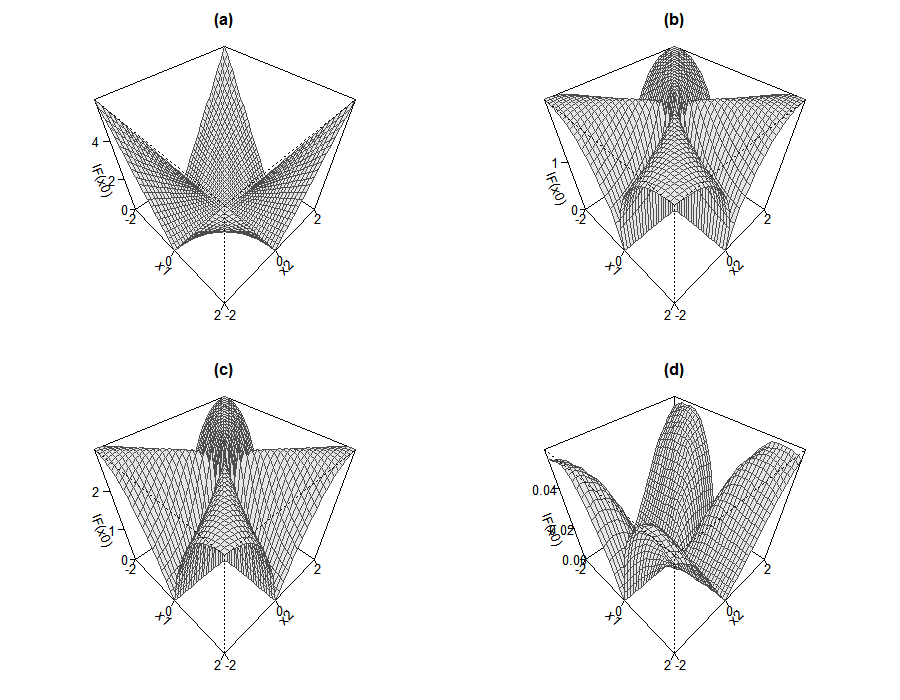
\includegraphics[height=12cm]{../Codes/IFnorm.png}
	\caption{Plot of the norm of influence function for first eigenvector of (a) sample covariance matrix, (b) SCM, (c) Tyler's scatter matrix and (d) Halfspace-DCM, for a bivariate normal distribution with $\bfmu = {\bf 0}, \Sigma = diag(2,1)$}
	\label{fig:IFnorm}
\end{figure}

\subsection{Asymptotic and finite-sample efficiencies}
Suppose $\hat\Sigma$ is a $\sqrt n$-consistent estimator of the population covariance matrix $\Sigma$, which permits a spectral decomposition $ \hat\Sigma = \hat\Gamma \hat\Lambda \hat\Gamma^T $, where $\hat\Gamma = (\hat\bfgamma_1,...,\hat\bfgamma_p)$. Then the asymptotic variance of the eigenvectors are (see Theorem 13.5.1 in \cite{anderson})
\begin{equation} \label{equation:covevEq}
AVar(\sqrt n\hat \bfgamma_i) = \sum_{k=1; k \neq i}^p \frac{\lambda_i \lambda_k}{(\lambda_i - \lambda_k)^2} \bfgamma_k \bfgamma_k^T
\end{equation}

the asymptotic relative efficiencies of eigenvectors from the sample DCM with respect to the sample covariance matrix can now be derived using (\ref{equation:covevEq}) above and (\ref{equation:DevEq}) from Corollary \ref{Corollary:eigendist}:
\begin{eqnarray*}
ARE(\hat\bfgamma^D_i, \hat\bfgamma_i; F) &=& \frac{Trace( AVar(\sqrt n\hat \bfgamma^D_i))}{Trace( AVar(\sqrt n\hat \bfgamma_i))}\\
&=& \left[\sum_{k=1; k \neq i}^p \frac{\lambda_i \lambda_k}{(\lambda_i - \lambda_k)^2} \right]^{-1} \left[ \sum_{k=1; k \neq i}^p \frac{\lambda_i \lambda_k }{(\lambda_{D,s,i} - \lambda_{D,S,k})^2} E \left( \frac{(\tilde D_\bfZ (\bfz))^4 z_i^2 z_k^2}{(\bfz^T \Lambda \bfz)^2} \right) \right]
\end{eqnarray*}

For 2 dimensions, this expression can be somewhat simplified. Suppose the two eigenvalues are $\lambda$ and $\rho\lambda$. In that case the eigenvalues of the DCM are
$$ \lambda_{D,S,1} = E \left( \frac{(D_\bfZ(\bfz))^2 z_1^2}{z_1^2 + \rho z_2^2} \right), \quad
\lambda_{D,S,2} = E \left( \frac{(D_\bfZ(\bfz))^2 \rho z_2^2}{z_1^2 + \rho z_2^2} \right) $$

and by simple algebra we get
$$ ARE(\hat\bfgamma^D_1, \hat\bfgamma_1; F) = ARE(\hat\bfgamma^D_2, \hat\bfgamma_2; F) = (1-\rho)^2 \frac{E \left( \frac{(D_\bfZ(\bfz))^4 z_1^2z_2^2}{(z_1^2 + \rho z_2^2)^2}\right)}{E^2 \left( \frac{(D_\bfZ(\bfz))^2 (z_1^2 - \rho z_2^2)}{(z_1^2 + \rho z_2^2)} \right)} $$

\section*{Appendix A: \textbf{Form of $V_{D,S}(F)$}}
First observe that for $F$ having covariance matrix $\Sigma = \Gamma\Lambda\Gamma^T$,
$$ V_{D,S}(F)  = (\Gamma \otimes \Gamma) V_{D,S}(F_\Lambda) (\Gamma \otimes \Gamma)^T$$
Where $F_\Lambda$ has the same elliptic distribution as $F$, but with covariance matrix $\Lambda$. Now,
\begin{eqnarray*}
V_{D,S} (F_\Lambda) &=& E \left[ vec \left\{ \frac{(\tilde D_\bfZ (\bfz))^2 \Lambda^{1/2} \bfz\bfz^T \Lambda^{1/2}}{\bfz^T\Lambda\bfz} - \Lambda_{D,S} \right\} vec^T \left\{ \frac{(\tilde D_\bfZ (\bfz))^2 \Lambda^{1/2} \bfz\bfz^T \Lambda^{1/2}}{\bfz^T\Lambda\bfz} - \Lambda_{D,S} \right\} \right]\\
&=& E \left[ vec \left\{ (\tilde D_\bfZ (\bfz))^2 SS(\Lambda^{1/2}\bfz; \bf0) \right\} vec^T \left\{ (\tilde D_\bfZ (\bfz))^2 SS(\Lambda^{1/2}\bfz; \bf0) \right\} \right]\\
&& - \quad vec(\Lambda_{D,S}) vec^T(\Lambda_{D,S})
\end{eqnarray*}

The matrix $vec(\Lambda_{D,S}) vec^T(\Lambda_{D,S})$ consists of elements $\lambda_i\lambda_j$ at $(i,j)^\text{th}$ position of the $(i,j)^\text{th}$ block, and 0 otherwise. These positions correspond to variance and covariance components of on-diagonal elements. For the expectation matrix, all its elements are of the form $E[\sqrt{\lambda_a \lambda_b \lambda_c \lambda_d} z_a z_b z_c z_d . (\tilde D_\bfZ (\bfz))^4 / (\bfz^T \Lambda \bfz)^2]$, with $1 \leq a,b,c,d \leq p$. Since $(\tilde D_\bfZ (\bfz))^4 / (\bfz^T \Lambda \bfz)^2$ is even in $\bfz$, which has a circularly symmetric distribution, all such expectations will be 0 unless $a=b=c=d$, or they are pairwise equal. Following a similar derivation for spatial sign covariance matrices in \cite{magyar14}, we collect the non-zero elements and write the matrix of expectations:
$$ (I_{p^2} + K_{p,p}) \left\{ \sum_{a=1}^p \sum_{b=1}^p \gamma^D_{ab} (\bfe_a \bfe_a^T \otimes  \bfe_b \bfe_b^T) - \sum_{a=1}^p \gamma^D_{aa} (\bfe_a \bfe_a^T \otimes  \bfe_a \bfe_a^T) \right\} + \sum_{a=1}^p \sum_{b=1}^p \gamma^D_{ab} (\bfe_a \bfe_b^T \otimes  \bfe_a \bfe_b^T) $$

where $I_k = (\bfe_1,...,\bfe_k), K_{m,n} = \sum_{i=1}^m \sum_{j=1}^n J_{ij} \otimes J_{ij}^T$ with $J_{ij}$ the $m \times n$ matrix having 1 as $(i,j)^\text{th}$ element and 0 elsewhere, and $\gamma^D_{mn} = E[ \lambda_m \lambda_n z_m^2 z_n ^2 . (\tilde D_\bfZ (\bfz))^4 / (\bfz^T \Lambda \bfz)^2]; 1 \leq m,n \leq p$.

\paragraph{}Putting everything together, denote $\hat S^D(F_\Lambda) = \sum_{i=1}^n (\tilde D^n_\bfZ (\bfz_i))^2 SS(\Lambda^{1/2}\bfz_i; \hat \bfmu_n)/n $. Then the different types of elements in the matrix $V_{D,S}(F_\Lambda)$ are as given below ($1 \leq a,b,c,d \leq p$):

\begin{itemize}
\item Variance of on-diagonal elements
$$ AVar( \sqrt n \hat S^D_{aa} (F_\Lambda)) = E \left[ \frac{(\tilde D_\bfZ (\bfz))^4 \lambda_a^2 z_a^4}{(\bfz^T \Lambda \bfz)^2} \right] - \lambda_{D,S,a}^2 $$

\item Variance of off-diagonal elements ($a \neq b$)
$$ AVar( \sqrt n \hat S^D_{ab} (F_\Lambda)) = E \left[ \frac{(\tilde D_\bfZ (\bfz))^4 \lambda_a \lambda_b z_a^2 z_b^2}{(\bfz^T \Lambda \bfz)^2} \right] $$

\item Covariance of two on-diagonal elements ($a \neq b$)
$$ ACov(\sqrt n \hat S^D_{aa} (F_\Lambda), \sqrt n \hat S^D_{bb} (F_\Lambda))
= E \left[ \frac{(\tilde D_\bfZ (\bfz))^4 \lambda_a \lambda_b z_a^2 z_b^2}{(\bfz^T \Lambda \bfz)^2} \right] - \lambda_{D,S,a} \lambda_{D,S,b} $$

\item Covariance of two off-diagonal elements ($a \neq b \neq c \neq d$)
$$ ACov(\sqrt n \hat S^D_{ab} (F_\Lambda), \sqrt n \hat S^D_{cd} (F_\Lambda)) = 0 $$

\item Covariance of one off-diagonal and one on-diagonal element ($a \neq b \neq c$)
$$ ACov(\sqrt n \hat S^D_{ab} (F_\Lambda), \sqrt n \hat S^D_{cc} (F_\Lambda)) = 0 $$
\end{itemize}

\section*{Appendix B: Proofs}
\begin{proof}[\textbf{Proof of Theorem  \ref{Theorem:covform}}]

\end{proof}

\begin{proof}[\textbf{Proof of Lemma \ref{Lemma:lemma1}}]
For two positive definite matrices $A,B$, we denote by $A>B$ that $A-B$ is positive definite. Also, denote
$$ S_n = \sqrt n \left[ \frac{1}{n} \sum_{i=1}^n \left| (\tilde D^{n} _\bfX (\bfx_i))^2  - (\tilde D_\bfX (\bfx_i))^2 \right| SS(\bfx_i; \hat\bfmu_n) \right] $$
Now, convergence in probability of $D^n_\bfX(.)$ to $D_\bfX(.)$ (hence $(\tilde D^n_\bfX(.))^2$ to $(\tilde D_\bfX(.))^2$) implies that given $\epsilon, \delta > 0$ there exists $N \in \mathbb{N}$ so that
\begin{eqnarray} \label{equation:lemma1eq}
\notag P \left[ |(\tilde D^{n_1}_\bfX(\bfx))^2 - (\tilde D_\bfX(\bfx))^2| > \epsilon \right] &<& \delta\\
\notag \Rightarrow \qquad |(\tilde D^{n_1}_\bfX(\bfx))^2 - (\tilde D_\bfX(\bfx))^2|
&<& \epsilon(1-\delta) + M\delta \\
&<& \epsilon + M\delta
\end{eqnarray}
for all $n_1 \geq N$, where $M$ is the largest value the square of a depth function can take. Consequently for all such $n_1$,
$$ S_{n_1} \quad < \quad
(\epsilon + M\delta) . \sqrt n_1 \left[ \frac{1}{n_1} \sum_{i=1}^{n_1} SS(\bfx_i; \hat\bfmu_{n_1}) \right] $$

We now construct a sequence of positive definite matrices $\{A_k (B_k+C_k) : k \in \mathbb N\} $ so that
$$ A_k = \frac{1+M}{k}, \quad B_k = \sqrt N_k \left[ \frac{1}{N_k} \sum_{i=1}^{N_k} \left\{ SS(\bfx_i; \hat\bfmu_{N_k}) - SS(\bfx_i; \bfmu) \right\} \right] $$
$$ \quad C_k = \sqrt N_k \left[ \frac{1}{N_k} \sum_{i=1}^{N_k} SS(\bfx_i; \bfmu) \right] $$

where $N_k \in \mathbb N$ gives the relation (\ref{equation:lemma1eq}) in place of $N$ when we take $\epsilon = \delta  =1/k$. Under conditions $ E\|\bfx - \bfmu\|^{-3/2} < \infty $ and $\sqrt n (\hat\bfmu_n - \bfmu) = O_P(1)$, the sample sign covariance matrix with unknown location parameter $\hat\bfmu_n$ has the same asymptotic distribution as the same with known location $\bfmu$ \citep{durre14}, hence $B_k \stackrel{P}{\rightarrow} 0$. Now by Slutsky's theorem, $A_k (B_k+C_k) \stackrel{P}{\rightarrow} 0$. Finally, for any $\epsilon_1 > 0$, $ P(S_{N_k} > \epsilon_1) < P(A_k B_k > \epsilon_1)$, hence the subsequence $\{S_{N_k}\} \stackrel{P}{\rightarrow} 0$. Since the main sequence $\{S_k\}$ is bounded below by 0, we have the needed.
\end{proof}

\begin{proof}[\textbf{Proof of Theorem \ref{Theorem:rootn}}]
The quantity in the statement of the theorem can be broken down as:
\begin{eqnarray*}
\sqrt n \left[ vec\left\{ \frac{1}{n} \sum_{i=1}^n (\tilde D^n_\bfX (\bfx_i))^2 SS(\bfx_i; \hat\bfmu_n) \right\} - vec\left\{ \frac{1}{n} \sum_{i=1}^n (\tilde D_\bfX (\bfx_i))^2 SS(\bfx_i; \bfmu) \right\} \right] +\\
\sqrt n \left[ vec\left\{ \frac{1}{n} \sum_{i=1}^n (\tilde D_\bfX (\bfx_i))^2 SS(\bfx_i; \bfmu) \right\} - E \left[ vec\left\{ (\tilde D_\bfX (\bfx))^2 SS(\bfx; \bfmu) \right\} \right] \right]
\end{eqnarray*}

The first part goes to 0 in probability by Lemma \ref{Lemma:lemma1}, and applying Slutsky's theorem we get the required convergence.
\end{proof}

\begin{proof}[\textbf{Proof of Theorem \ref{Theorem:decomp}}]
See \cite{taskinen12}
\end{proof}

\begin{proof}[\textbf{Proof of Corollary \ref{Corollary:eigendist}}]
In spirit, this corollary is similar to Theorem 13.5.1 in \cite{anderson}, and indeed, \cite{taskinen12} used this theorem to prove Theorem \ref{Theorem:decomp}. Due to the decomposition (\ref{equation:decompEq}) we have, for the distribution $F_\Lambda$, the following relation between any off-diagonal element of $\hat S^D(F_\Lambda)$ and the corresponding element in the estimate of eigenvectors $\hat\Gamma_D (F_\Lambda)$:

$$ \sqrt n \hat\gamma_{D,ij} (F_\Lambda) = \sqrt n \frac{\hat S^D_{ij} (F_\Lambda)}{\lambda_{D,S,i} - \lambda_{D,S,j}}; \quad i \neq j$$

So that for eigenvector estimates of the original $F$ we have
\begin{equation} \label{equation:app1}
\sqrt n (\hat\bfgamma_{D,i} - \bfgamma_i) = \sqrt n \Gamma (\hat \bfgamma_{D,i}(F_\Lambda) - \bfe_i ) = \sqrt n \left[ \sum_{k=1; k \neq i}^p \hat \gamma_{D,ik}(F_\Lambda)\bfgamma_k + (\hat \gamma_{D,ii}(F_\Lambda) - 1)\bfgamma_i \right] \tag{A1}
\end{equation}

$\sqrt n (\hat \gamma_{D,ii}(F_\Lambda) - 1) =  o_P(1)$ and $ACov(\sqrt n \hat S^D_{ik}(F_\Lambda), \sqrt n \hat S^D_{il}(F_\Lambda)) = 0$ for $k \neq l$, so the above equation implies

$$ AVar(\bfg_i) = AVar (\sqrt n (\hat\bfgamma_{D,i} - \bfgamma_i)) = \sum_{k=1; k \neq i}^p \frac{AVar(\sqrt n \hat S^D_{ik}(F_\Lambda))}{(\lambda_{D,s,i} - \lambda_{D,S,k})^2} \bfgamma_k \bfgamma_k^T $$

For the covariance terms, from (\ref{equation:app1}) we get, for $i \neq j$,
\begin{eqnarray*}
ACov(\bfg_i, \bfg_j) &=& ACov (\sqrt n (\hat\bfgamma_{D,i} - \bfgamma_i), \sqrt n (\hat\bfgamma_{D,j} - \bfgamma_j))\\
&=& ACov \left( \sum_{k=1; k \neq i}^p \sqrt n \hat \gamma_{D,ik}(F_\Lambda)\bfgamma_k, \sum_{k=1; k \neq j}^p \sqrt n \hat \gamma_{D,jk}(F_\Lambda)\bfgamma_k \right)\\
&=& ACov \left( \sqrt n \hat \gamma_{D,ij}(F_\Lambda)\bfgamma_j, \sqrt n \hat \gamma_{D,ji}(F_\Lambda)\bfgamma_i \right)\\
&=& - \frac{AVar(\sqrt n \hat S^D_{ij}(\Lambda))}{(\lambda_{D,s,i} - \lambda_{D,S,j})^2} \bfgamma_j \bfgamma_i^T
\end{eqnarray*}

The exact forms given in the statement of the corollary now follows from the  Form of $V_{D,S}$ in Appendix A.

\paragraph{}For the on-diagonal elements of $\hat S^D(F_\Lambda)$ Theorem \ref{Theorem:decomp} gives us $ \sqrt n \hat\lambda_{D,s,i} (F_\Lambda) = \sqrt n \hat S^D_{ii}(F_\Lambda)$ for $i = 1,...,p$. Hence
\begin{eqnarray*}
AVar(l_i) &=& AVar(\sqrt n \hat\lambda_{D,s,i} - \sqrt n \lambda_{D,S,i})\\
&=& AVar(\sqrt n \hat\lambda_{D,s,i} (F_\Lambda) - \sqrt n \lambda_{D,S,i}(F_\Lambda))\\
&=& AVar(\sqrt n S^D_{ii}(F_\Lambda))
\end{eqnarray*}

A similar derivation gives the expression for $AVar(l_i,l_j); i \neq j$. Finally, since the asymptotic covariance between an on-diagonal and an off-diagonal element of $\hat S^D(F_\Lambda)$, it follows that the elements of $G$ and diagonal elements of $L$ are independent.
\end{proof}

\bibliographystyle{plainnat}
\bibliography{scatterbib}

\end{document}